\section{Downstream Embodied Case Study: Closed-Loop Navigation (\textbf{RQ4})}
\label{sec:navigation}

While static grounding isolates single-step perceptual sensitivity, embodied policies integrate visual observations sequentially across dozens of control steps. We therefore extend our analysis to closed-loop Vision-and-Language Navigation (\textsc{VLN}) using \textsc{InternNav/DualVLN} \citep{Wei2026Ground} over three unseen KuJiaLe indoor apartment scenes (\texttt{0031}, \texttt{0036}, \texttt{0066}; 33 paired episodes per scene, totaling 99 paired episodes and 198 closed-loop rollouts).

\paragraph{Task setup and evaluation metrics}
In each episode, the embodied agent receives a natural-language navigation instruction and egocentric RGB frames rendered continuously from either the \original\ (\textsc{MDL}) or \converted\ (\usdps) scene graph, holding the starting pose, goal region, maximum step budget, and stopping rule fixed (the policy explicitly invokes \texttt{STOP} within the evaluator's success radius without oracle termination). Following standard \textsc{VLN} practice \citep{Anderson2018Vision}, we report binary Success Rate (\textsc{SR}), Success weighted by Path Length ($\mathrm{SPL} = S \cdot L^*/\max(L, L^*)$, where $L$ is executed path length and $L^*$ is shortest-path geodesic length), Navigation Error (\textsc{NE}, final Euclidean distance to the goal in meters), and Trajectory Length (\textsc{TL}).

\begin{table}[!t]
\centering\scriptsize
% Generated from optical_mechanisms & navigation JSONs
\begin{tabular*}{\columnwidth}{@{\extracolsep{\fill}}lrrrrrr@{}}
\toprule
Scene & $N$ & $\mathrm{SR}_O$ & $\mathrm{SR}_C$ & $\mathrm{SPL}_O$ & $\mathrm{SPL}_C$ & Flips \\
\midrule
\texttt{0031} & 33 & 51.5 & 57.6 & 47.9 & 49.6 & 8 \\
\texttt{0036} & 33 & 81.8 & 60.6 & 70.0 & 55.0 & 11 \\
\texttt{0066} & 33 & 24.2 & 27.3 & 24.2 & 24.3 & 11 \\
\midrule
All & 99 & 52.5 & 48.5 & 47.4 & 43.0 & 30 \\
\bottomrule
\end{tabular*}

\caption{Paired closed-loop \textsc{InternNav/DualVLN} navigation outcomes across three KuJiaLe \texttt{val\_unseen} scenes (33 episodes per scene, 99 pairs). \textsc{SR} and \textsc{SPL} are percentages; $O$ and $C$ denote \original\ and \converted\ materials.}
\label{tab:navigation}
\end{table}

\begin{figure*}[!t]
\centering
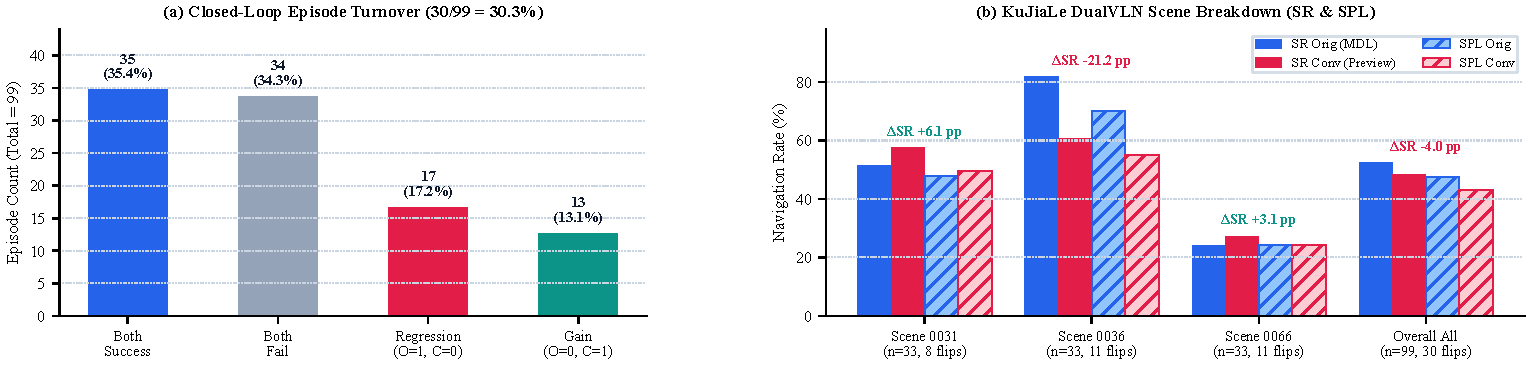
\includegraphics[width=\textwidth]{fig6_navigation_vln.pdf}
\caption{\textbf{Closed-loop \textsc{InternNav/DualVLN} navigation outcome redistribution over 99 paired episodes (\textbf{RQ4}).}
\emph{(a)} Aggregate outcome transitions: 17 success-to-failure losses and 13 failure-to-success gains yield 30 changed episode outcomes ($30.3\%$ turnover) despite only a $-4.0$ percentage-point net \textsc{SR} shift ($52.5\% \to 48.5\%$).
\emph{(b)} Scene-level \textsc{SR} and \textsc{SPL} breakdown across scenes \texttt{0031}, \texttt{0036}, and \texttt{0066}.}
\label{fig:navigation}
\end{figure*}

\paragraph{Bidirectional outcome redistribution across trajectories}
Table~\ref{tab:navigation} and Figure~\ref{fig:navigation} reveal the same aggregate cancellation pattern observed in single-frame grounding, amplified over multi-step closed-loop rollouts. Aggregate \textsc{SR} moves modestly from \NavSrOriginal\% ($52/99$) to \NavSrConverted\% ($48/99$, net $-4.0$ pp), while mean \textsc{NE} ($3.680 \to 3.631$) and \textsc{TL} ($6.975 \to 7.060$) barely change. At the episode level, however, \NavFlips/\NavN\ episodes (\NavFlipPercent\%) change final binary status: 17 previously successful episodes fail while 13 previously unsuccessful episodes succeed. Scene \texttt{0036} suffers the sharpest drop ($81.8\% \to 60.6\%$ \textsc{SR}, $-15.0$ pp \textsc{SPL}), whereas scenes \texttt{0031} and \texttt{0066} show net increases ($+6.1$ pp and $+3.1$ pp \textsc{SR}). Fresh simulator load profiling across 18 launches (\ref{app:navigation}) confirms comparable initialization timing and GPU memory utilization under both shader pipelines.

\paragraph{Qualitative trajectory divergence}
Figure~\ref{fig:trajectories} presents ending observations and top-down path overlays from dedicated qualitative video recordings of three paired episodes (expanded to 12 paired recordings in \ref{app:navigation}). Early visual discrepancies near reflective doorways and hallways compound across action steps, shifting turn selection and triggering premature or delayed \texttt{STOP} decisions. Together with Table~\ref{tab:navigation}, these trajectories illustrate how shader-level changes alter sequential control; isolating shader effects from multi-run simulator variance across repeated closed-loop rollouts remains a practical direction noted in Section~\ref{sec:conclusion}.

\begin{figure}[!t]
\centering
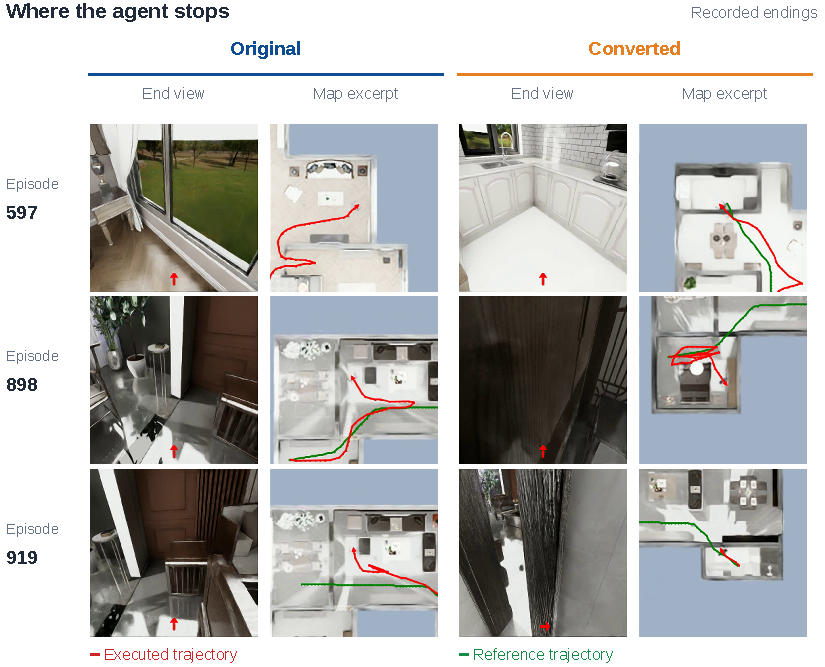
\includegraphics[width=\linewidth]{trajectories.pdf}
\caption{Qualitative ending views and top-down trajectory excerpts from separate video reruns sharing episode IDs with the 99-pair evaluation. Red and green paths trace executed and reference trajectories.}
\label{fig:trajectories}
\end{figure}
